\documentclass[11pt,a4paper]{article}

\usepackage{amsmath}
\usepackage{amsthm}
\usepackage{amssymb}
\usepackage{booktabs}
\usepackage{graphicx}
\usepackage{color}
\usepackage{fullpage}
\usepackage{listings}
\usepackage{color}
\usepackage{url}
\usepackage{multirow}
\usepackage{forest}
% 為了讓表格緊密
\usepackage{float}
% 為了首行空格
%\usepackage{indentfirst}
% % 為表格添加 footnote
% \usepackage{tablefootnote}

\usepackage{tabularx}

% 全域格式設定（放在 preamble）
\lstset{
  numbers=left,
  numberstyle=\tiny\color{gray},
  stepnumber=1,
  numbersep=5pt,
  frame=single,
  basicstyle=\ttfamily\small,
  breaklines=true,
  showspaces=false,        % ← 明確關掉，確保空格不顯示為 ␣
  showstringspaces=false   % ← 字串內的空格也不顯示為 ␣
}

% 語言定義只放語言相關設定
\lstdefinelanguage{JavaScript}{
  keywords={break, case, ...},
  morekeywords=[2]{class, const, ...},
  sensitive=true,
  morecomment=[l]{//},
  morecomment=[s]{/*}{*/},
  morestring=[b]',
  morestring=[b]"
}

\lstdefinelanguage{Bash}{
  keywords={cd, npm, npx, ...},
  sensitive=true,
  morestring=[b]',
  morestring=[b]"
}

% for Chinese
\usepackage{fontspec} % 加這個就可以設定字體
\usepackage[BoldFont, SlantFont]{xeCJK} % 讓中英文字體分開設置
\setCJKmainfont{Microsoft JhengHei}  % 設定中文為系統上的字型，而英文不去更動，使用原TeX字型
\setCJKmonofont{Microsoft JhengHei} % 定義 CJK 等寬字型，避免 xeCJK 無法識別 \CJKttdefault
\renewcommand{\baselinestretch}{1.3}

\parskip=5pt
\parindent=24pt
\newtheorem{lemma}{Lemma}
\newtheorem{ques}{Question}
\newtheorem{prop}{Proposition}
\newtheorem{defn}{Definition}
\newtheorem{rmk}{Remark}
\newtheorem{note}{Note}
\newtheorem{eg}{Example}
\newtheorem{aspt}{Assumption}

\definecolor{emphOrange}{RGB}{247, 80, 0}
\definecolor{stringGray}{RGB}{109, 109, 109}
\definecolor{commentGreen}{RGB}{0, 96, 0}
\definecolor{mygreen}{rgb}{0,0.6,0}
\definecolor{mygray}{rgb}{0.5,0.5,0.5}
\definecolor{mymauve}{rgb}{0.58,0,0.82}



% "摘要", "表", "圖", "參考文獻"
\renewcommand{\abstractname}{\bf 摘要}
\renewcommand{\tablename}{表}
\renewcommand{\figurename}{圖}
\renewcommand{\refname}{\bf 參考文獻}

% -----
% 我在這裡加入了 tikz 和 forest 宏包 (基於 tikz) 來繪製 B+ Tree
\usepackage{tikz} % <<< --- 新增：明確載入 tikz
\usepackage{forest}
\usetikzlibrary{arrows.meta, chains}
% -----


\begin{document}

\title{雲原生 HW3 - Testing}
\author{資管三 B12705041 李倢安}
\date{\today}
\maketitle
%\fontsize{20}{20pt}\selectfont

\section*{Test 1：Backend — POST /api/v1/todos 成功建立 Todo}

\subsection*{測試檔案：} 
\texttt{backend/test/todo.post.spec.ts}

\begin{lstlisting}[language=JavaScript]
import { afterAll, afterEach, beforeAll, describe, expect, test, vi } from 'vitest'
import { serverOf } from '../src/server'
import * as TodoRepo from '../src/repo/todo'
import { FastifyInstance } from 'fastify'
import { Todo } from '../src/types/todo'

describe('Todo POST API Testing', () => {
  let server: FastifyInstance

  beforeAll(async () => {
    server = serverOf()
    await server.ready()
  })

  afterAll(async () => {
    await server.close()
  })

  afterEach(() => {
    vi.resetAllMocks()
  })

  test('Given valid name and description, When receive a POST /api/v1/todos request, Then it should response with status code 201 and the created todo', async () => {
    // arrange: mock the repo function to return the created todo
    const createdTodo: Todo = {
      id: 'mock-id-1',
      name: 'Buy groceries',
      description: 'Go to the supermarket',
      status: false
    }
    const createSpy = vi.spyOn(TodoRepo, 'createTodo').mockResolvedValue(createdTodo)

    // act: send POST /api/v1/todos with valid body
    const response = await server.inject({
      method: 'POST',
      url: '/api/v1/todos',
      payload: JSON.stringify({ name: 'Buy groceries', description: 'Go to the supermarket' }),
      headers: { 'Content-Type': 'application/json' }
    })

    // assert: status 201 and body contains the created todo
    expect(response.statusCode).toBe(201)
    const result = JSON.parse(response.body)['todo']
    expect(result).toStrictEqual(createdTodo)

    // assert: repo was called exactly once with the correct payload
    expect(createSpy).toHaveBeenCalledTimes(1)
    expect(createSpy).toHaveBeenCalledWith(
      expect.objectContaining({ name: 'Buy groceries', description: 'Go to the supermarket' })
    )
  })

  test('Given the repo throws an error, When receive a POST /api/v1/todos request, Then it should response with status code 500', async () => {
    // arrange: mock the repo to throw
    vi.spyOn(TodoRepo, 'createTodo').mockRejectedValue(new Error('DB connection failed'))

    // act
    const response = await server.inject({
      method: 'POST',
      url: '/api/v1/todos',
      payload: JSON.stringify({ name: 'Buy groceries', description: 'Go to the supermarket' }),
      headers: { 'Content-Type': 'application/json' }
    })

    // assert: server should swallow the error and return 500
    expect(response.statusCode).toBe(500)
  })
})

\end{lstlisting}

\subsection*{測試報告截圖如下：}
\begin{figure}[H]
    \centering
    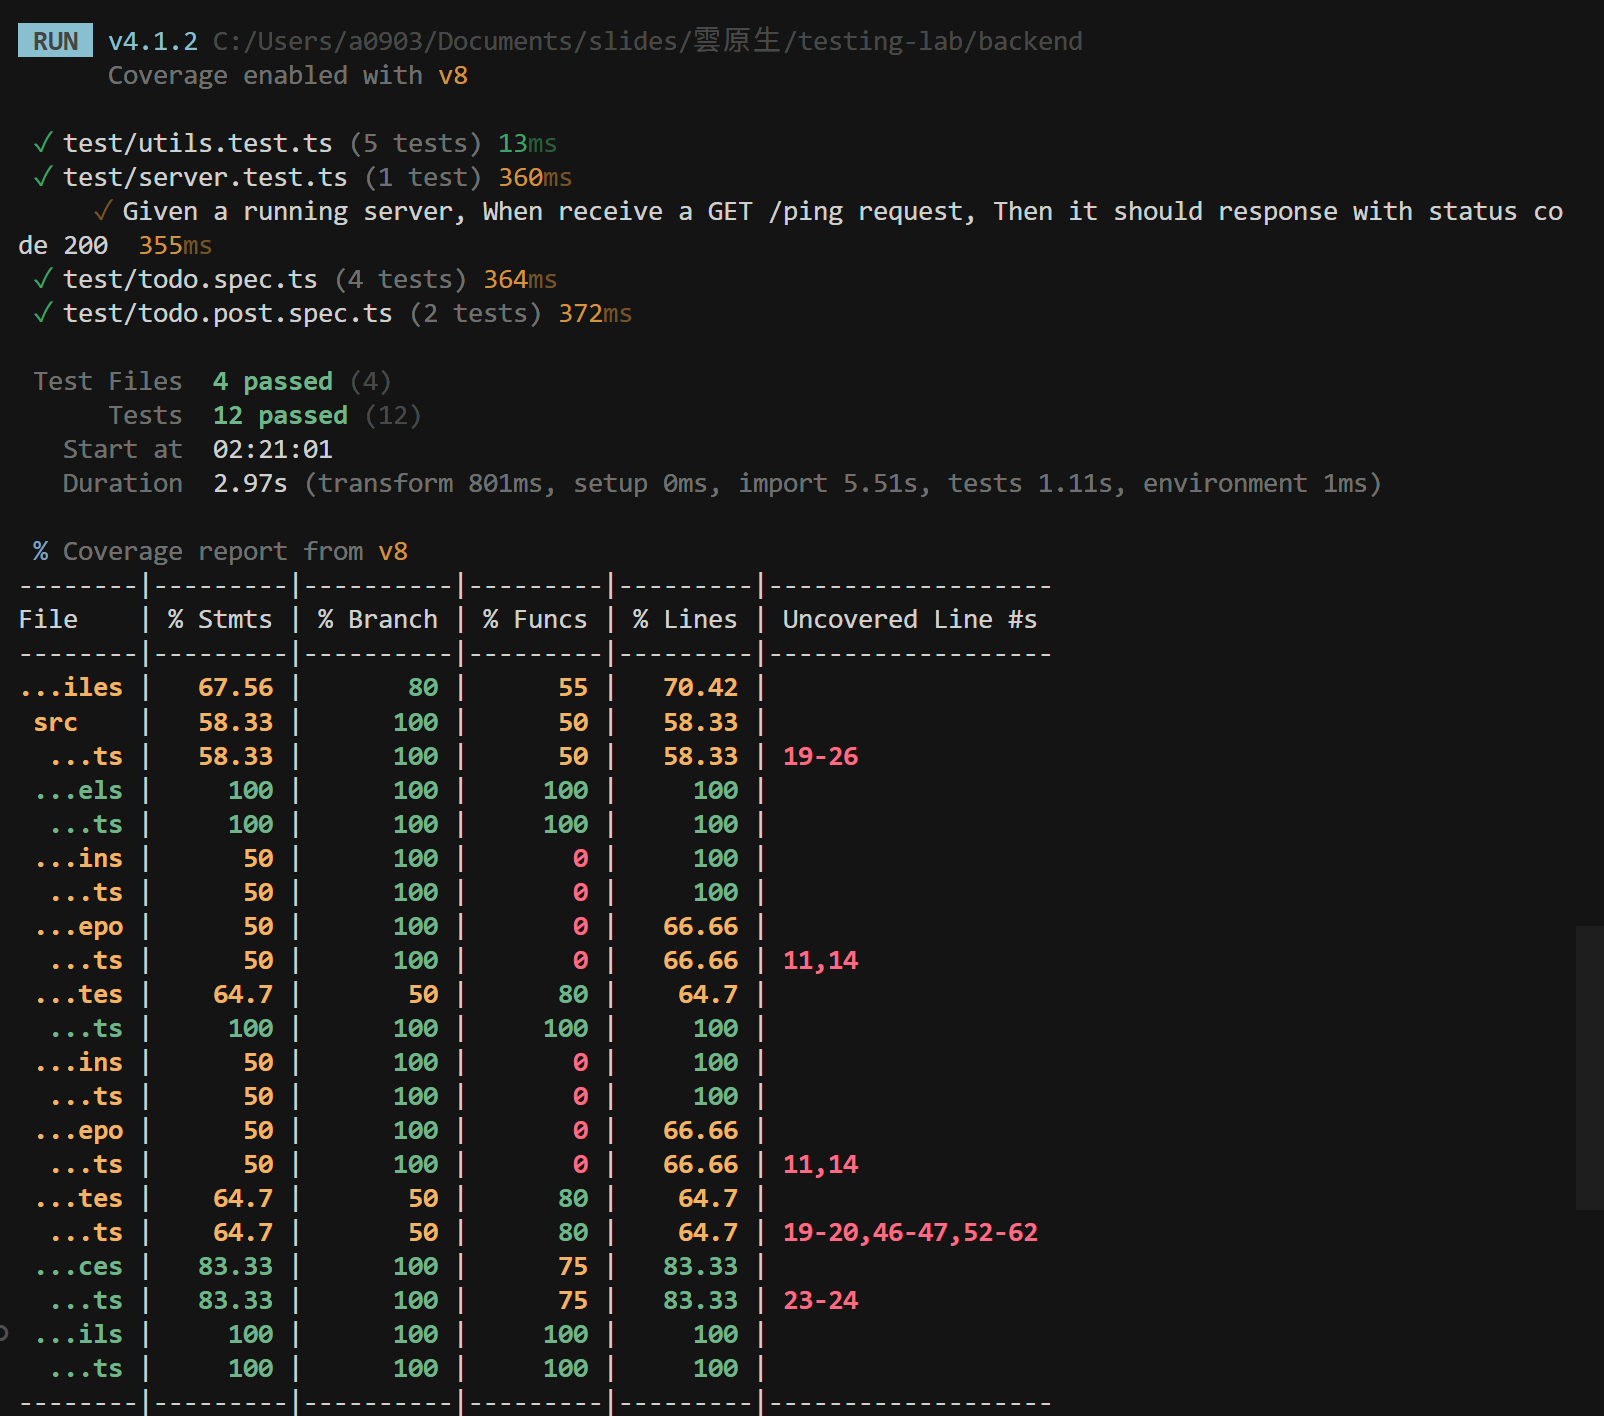
\includegraphics[width=0.8\textwidth]{todo.post.spec.ts_implement.png}
    \caption{todo.post.spec.ts測試報告}
    \label{fig:todo_post_test_report}
\end{figure}


\subsection*{說明：}

測試工具\\
\begin{tabularx}{\linewidth}{@{}llllX@{}}
\toprule
層級 & 工具 & 版本 & 用途 \\
\midrule
Backend & Vitest & v4.1.2 & 單元 / 整合測試框架 \\
Backend & \texttt{@vitest/coverage-v8} & v4.1.2 & 程式碼覆蓋率報告 \\
Backend & Fastify \texttt{server.inject()} & — & 不需啟動真實 HTTP 伺服器即可發送請求 \\
\bottomrule
\end{tabularx}
\\
測試場景（Given / When / Then）\\
\begin{tabularx}{\linewidth}{@{}lX@{}}
\toprule
角色 & 說明 \\
\midrule
\textbf{Given} & 使用 \texttt{vi.spyOn(TodoRepo, 'createTodo').mockResolvedValue(...)} 模擬資料庫寫入，不需連接真實 MongoDB \\
\textbf{When} & 透過 \texttt{server.inject()} 對 \texttt{POST /api/v1/todos} 送出包含 \texttt{name} 與 \texttt{description} 的 JSON body \\
\textbf{Then} & HTTP status 為 201，response body 的 \texttt{todo} 欄位與 mock 回傳值完全一致；且 \texttt{createTodo} 恰好被呼叫一次，且呼叫參數包含正確的欄位 \\
\bottomrule
\end{tabularx}

\begin{itemize}

\item 測試主體：\texttt{TodoRouter}（路由層）→ \texttt{addTodo} service（服務層），資料層以 spy 隔離

\item Mock / 隔離策略：
    \begin{itemize}
        \item 使用 \texttt{vi.spyOn} 替換 \texttt{TodoRepo.createTodo}，完全跳過 Mongoose / MongoDB
        \item \texttt{afterEach} 呼叫 \texttt{vi.resetAllMocks()}，確保各測試案例互不干擾
        \item \texttt{server.inject()} 在記憶體內模擬 HTTP 請求，不需啟動網路監聽，測試速度快且無副作用
    \end{itemize}

\item 想驗證的東西：
    \begin{enumerate}
        \item 路由是否正確將 request body 傳遞給 service，再由 service 傳給 repo
        \item 成功建立時回傳 HTTP 201（而不是 200）
        \item response body 結構正確（包在 `todo` key 下）
        \item \texttt{createTodo} 被呼叫的次數與參數正確（防止漏呼叫或傳錯參數）
    \end{enumerate}
\end{itemize}

執行指令：
\begin{lstlisting}[language=Bash]
cd backend
npm test
\end{lstlisting}




\section*{Test 2：Frontend E2E — 點擊 Complete 後 Todo 切換至完成狀態}

\subsection*{測試檔案：} 
\texttt{frontend/tests/todo.spec.ts} （第 91 行起）

\begin{lstlisting}[language=JavaScript]
test('Given a todo with status false, When click Complete, Then the todo title should have line-through style and Complete button should be hidden', async ({ page }) => {
        const todo = {
            id: 'mock-id-complete',
            name: 'Exercise',
            description: 'Go for a run',
            status: false,
        };
        const completedTodo = { ...todo, status: true };

        // 1. Mock initial GET: return one incomplete todo
        await page.route('**/api/v1/todos', async (route) => {
            await route.fulfill({
                status: 200,
                contentType: 'application/json',
                body: JSON.stringify({ todos: [todo] }),
            });
        });

        // 2. Mock PUT (update status) → 200
        await page.route(`**/api/v1/todos/${todo.id}`, async (route) => {
            if (route.request().method() === 'PUT') {
                await route.fulfill({
                    status: 200,
                    contentType: 'application/json',
                    body: JSON.stringify({ todo: completedTodo }),
                });
            }
        });

        await page.goto(BASE_URL);

        // 3. Verify the todo is initially visible with no line-through
        const heading = page.getByRole('heading', { name: 'Exercise' });
        await expect(heading).toBeVisible();
        await expect(heading).not.toHaveClass('line-through');

        // 4. Re-route GET to return the completed todo before clicking Complete
        await page.route('**/api/v1/todos', async (route) => {
            await route.fulfill({
                status: 200,
                contentType: 'application/json',
                body: JSON.stringify({ todos: [completedTodo] }),
            });
        });

        // 5. Click Complete button
        await page.getByRole('button', { name: 'Complete' }).click();

        // 6. Assert: title has line-through CSS class
        await expect(heading).toHaveClass('line-through');

        // 7. Assert: Complete button is hidden (has hide-button class, which sets display:none)
        const completeButton = page.locator('button', { hasText: 'Complete' });
        await expect(completeButton).toBeHidden();
    });
\end{lstlisting}


\subsection*{測試報告截圖如下：}
\begin{figure}[H]
    \centering
    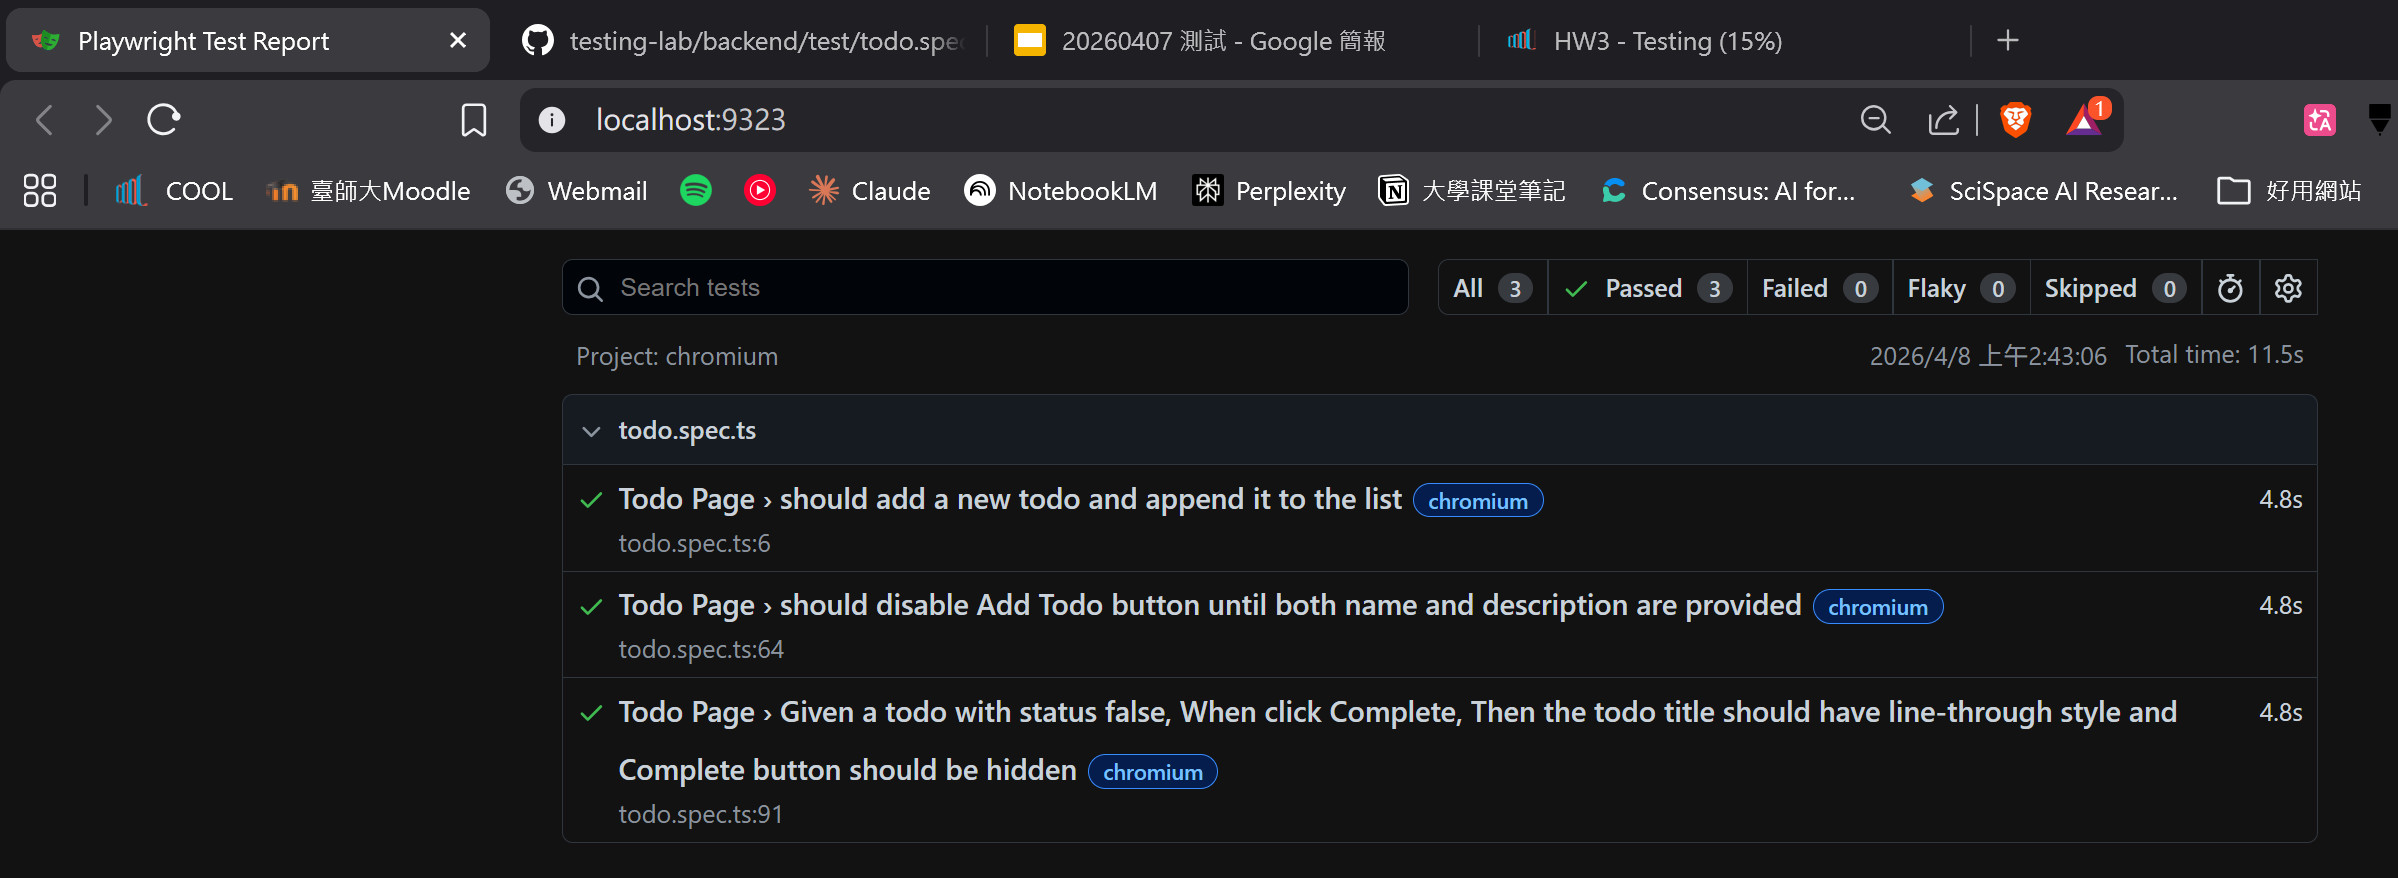
\includegraphics[width=0.8\textwidth]{frontend_test.png}
    \caption{todo.spec.ts E2E 測試報告}
    \label{fig:todo_e2e_test_report}
\end{figure}

\subsection*{說明：}
測試工具\\
\begin{tabularx}{\linewidth}{@{}llllX@{}}
\toprule
層級 & 工具 & 版本 & 用途 \\
\midrule
Frontend & Playwright & v1.51.0 & End-to-End 瀏覽器自動化測試框架 \\
Frontend & Playwright \texttt{page.route()} & — & 攔截並 mock 瀏覽器發出的 API 請求 \\
\bottomrule
\end{tabularx}
\\
測試場景（Given / When / Then）\\
\begin{tabularx}{\linewidth}{@{}lX@{}}
\toprule
角色 & 說明 \\
\midrule
\textbf{Given} & 以 \texttt{page.route('**/api/v1/todos', ...)} mock 初始 GET 回傳 1 筆 \texttt{status:false} 的 Todo，頁面載入後即看到 "Exercise" 項目，標題無刪除線 \\
\textbf{When} & 對 \texttt{PUT /api/v1/todos/:id} route 注入 200 回應；再更新 GET mock 回傳 \texttt{status:true}；最後點擊 \texttt{Complete} 按鈕觸發 \texttt{updateTodo()} → \texttt{fetchTodos()} \\
\textbf{Then} & 標題 \texttt{<h1>} 套用 CSS class \texttt{line-through}（文字顯示刪除線）；\texttt{Complete} 按鈕取得 class \texttt{hide-button}（\texttt{display:none}），\texttt{toBeHidden()} 通過 \\
\bottomrule
\end{tabularx}


\begin{itemize}
\item 測試主體：React 元件 \texttt{TodoItem}（\texttt{Complete} 按鈕、標題/描述的 class 邏輯）+ \texttt{App}（\texttt{handleUpdateTodo} 流程） + API 互動（\texttt{axios PUT → GET}）

\item Mock / 隔離策略：
    \begin{itemize}
        \item \texttt{page.route()} 在瀏覽器層攔截 API 呼叫，完全不需要真實 Backend 或 MongoDB
        \item 分兩階段 mock GET：第一階段回傳未完成狀態（初始渲染）、第二階段回傳完成狀態（點擊後 refetch）
        \item 每個測試案例各自設置 route handler，Playwright 自動在測試結束後清除
    \end{itemize}

\item 想驗證的東西：
    \begin{enumerate}
        \item 初始狀態：頁面正確渲染 \texttt{status:false} 的 Todo，無刪除線
        \item 點擊 \texttt{Complete} 後：UI 正確根據 \texttt{status:true} 套用 \texttt{line-through} class（視覺反饋）
        \item 點擊 \texttt{Complete} 後：\texttt{Complete} 按鈕被 CSS class \texttt{hide-button}（\texttt{display:none}）隱藏，防止重複點擊
        \item 驗證整個 UI 更新流程：\texttt{click → PUT API → GET refetch → React 重新渲染} 的完整鏈路
    \end{enumerate}
\end{itemize}

執行指令：
\begin{lstlisting}[language=Bash]
# 終端機 1：啟動前端 dev server
cd frontend
npm run dev

# 終端機 2：執行 E2E 測試
cd frontend
npx playwright test --project=chromium tests/todo.spec.ts

# 產生並開啟 HTML 報告
npx playwright show-report
\end{lstlisting}



\section*{實作1：修復測試}


\paragraph*{答:}

在實作1中，我們發現了utils.test.ts中的fabonacci testing未實作，導致測試失敗。為了修復這個問題，我們需要實作fabonacci function並確保它能正確計算斐波那契數列。
以下是修復後的utils.test.ts中fabonacci function 程式碼片段：
\begin{lstlisting}[language=JavaScript]
  describe('fabonacci testing', () => {
    it('should return 1 when n is 1', () => {
      expect(fabonacci(1)).toBe(1)
    })
    it('should return 1 when n is 2', () => {
      // arrange
      const n = 2

      // act
      const actual = fabonacci(n)

      // assert
      expect(actual).toBe(1)
    })
    it('should return 2 when n is 3', () => {
      // arrange
      const n = 3

      // act
      const actual = fabonacci(n)

      // assert
      expect(actual).toBe(2)
    })
  })
\end{lstlisting}

\subsection*{測試報告截圖如下：}
\begin{figure}[H]
    \centering
    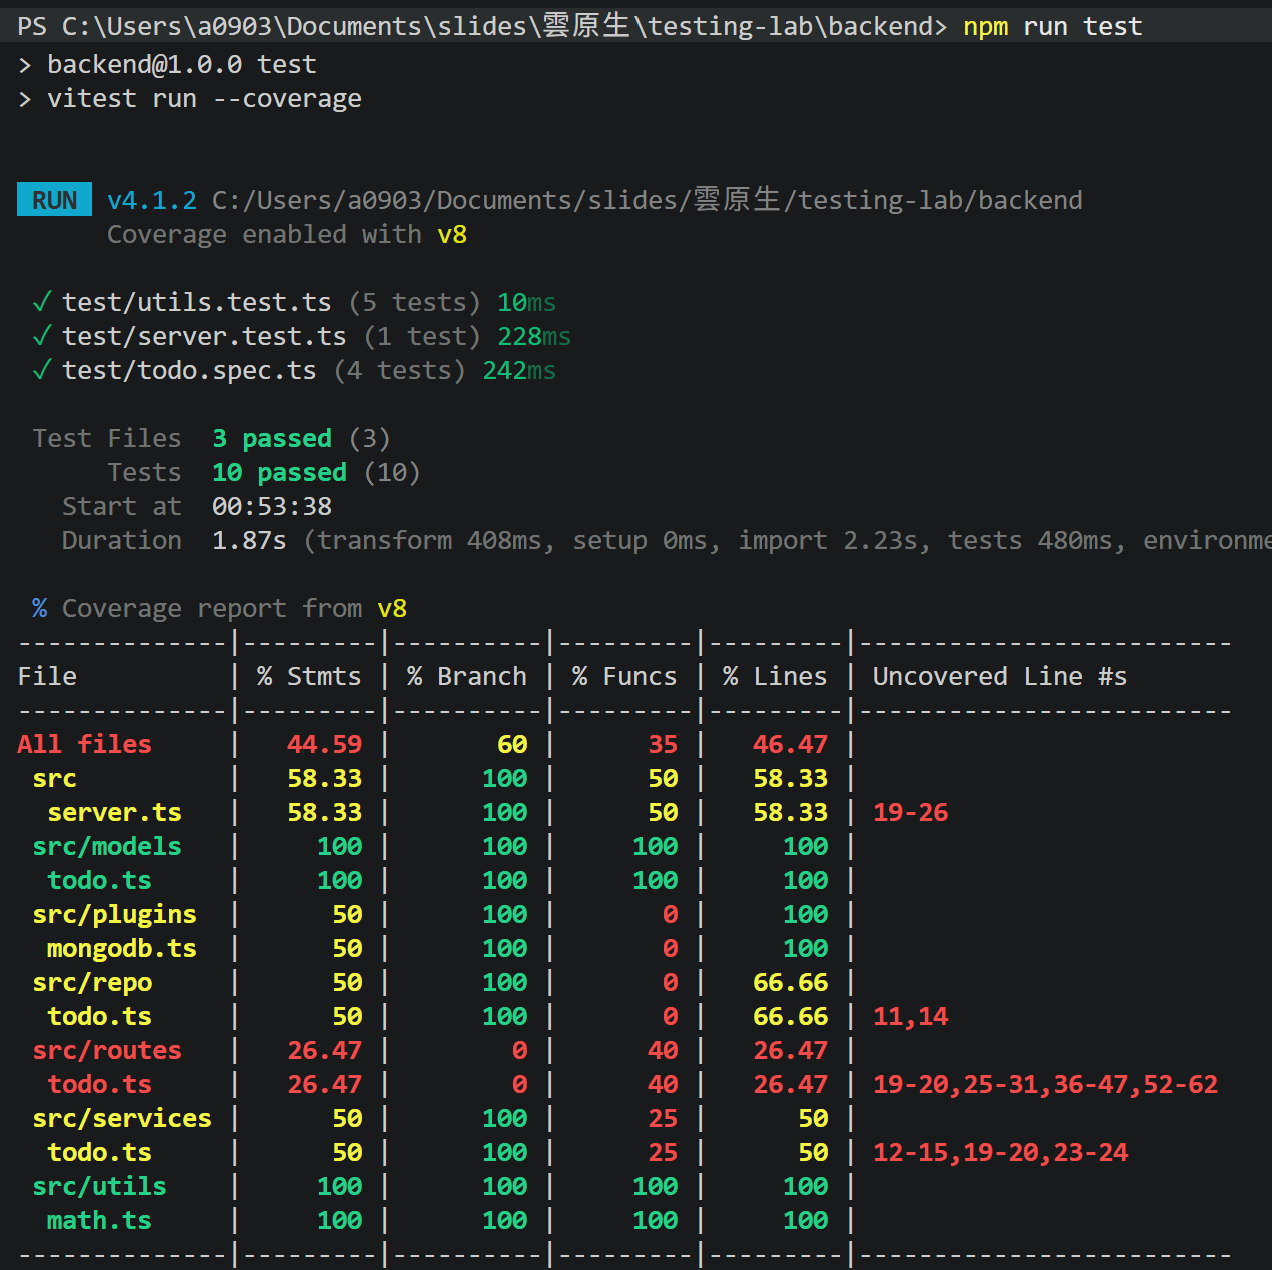
\includegraphics[width=0.8\textwidth]{fabonacci_testing_implement.png}
    \caption{修復後的fabonacci testing報告}
    \label{fig:test_report}
\end{figure}

\section*{實作2：透過AI協助你完成todo.spec.ts裡的測試}
\paragraph*{答:}
以下是修復後的todo.spec.ts中的程式碼片段：
\begin{lstlisting}[language=JavaScript]
    test('Given a valid ID and status, When receive a PUT /api/v1/todos/:id request, Then it should response the updated todo object', async () => {
    // arrange: mock the repo function to return an updated todo object
    const updatedTodo = {
      id: '1',
      name: 'todo 1',
      description: 'description 1',
      status: true
    }
    vi.spyOn(TodoRepo, 'updateTodoById').mockImplementation(async (id, status) => {
      if (id === '1') {
        return { ...updatedTodo }
      }
      return null
    })

    // act: receive a PUT /api/v1/todos/:id request
    const response = await server.inject({
      method: 'PUT',
      url: '/api/v1/todos/1',
      payload: JSON.stringify({ status: true }),
      headers: { 'Content-Type': 'application/json' }
    })

    // assert: response should be the updated todo object
    expect(response.statusCode).toBe(200)
    const result = JSON.parse(response.body)['todo']
    expect(result).toStrictEqual(updatedTodo)
  })

  test('Given an invalid ID, When receive a PUT /api/v1/todos/:id request, Then it should response with status code 404', async () => {
    // arrange: mock the repo function to return null
    vi.spyOn(TodoRepo, 'updateTodoById').mockImplementation(async (id, status) => {
      return null
    })

    // act: receive a PUT /api/v1/todos/:id request
    const response = await server.inject({
      method: 'PUT',
      url: '/api/v1/todos/does-not-exist',
      payload: JSON.stringify({ status: false }),
      headers: { 'Content-Type': 'application/json' }
    })

    // assert: response should with status code 404
    expect(response.statusCode).toBe(404)
  })

\end{lstlisting}

\subsection*{測試報告截圖如下：}
\begin{figure}[H]
    \centering
    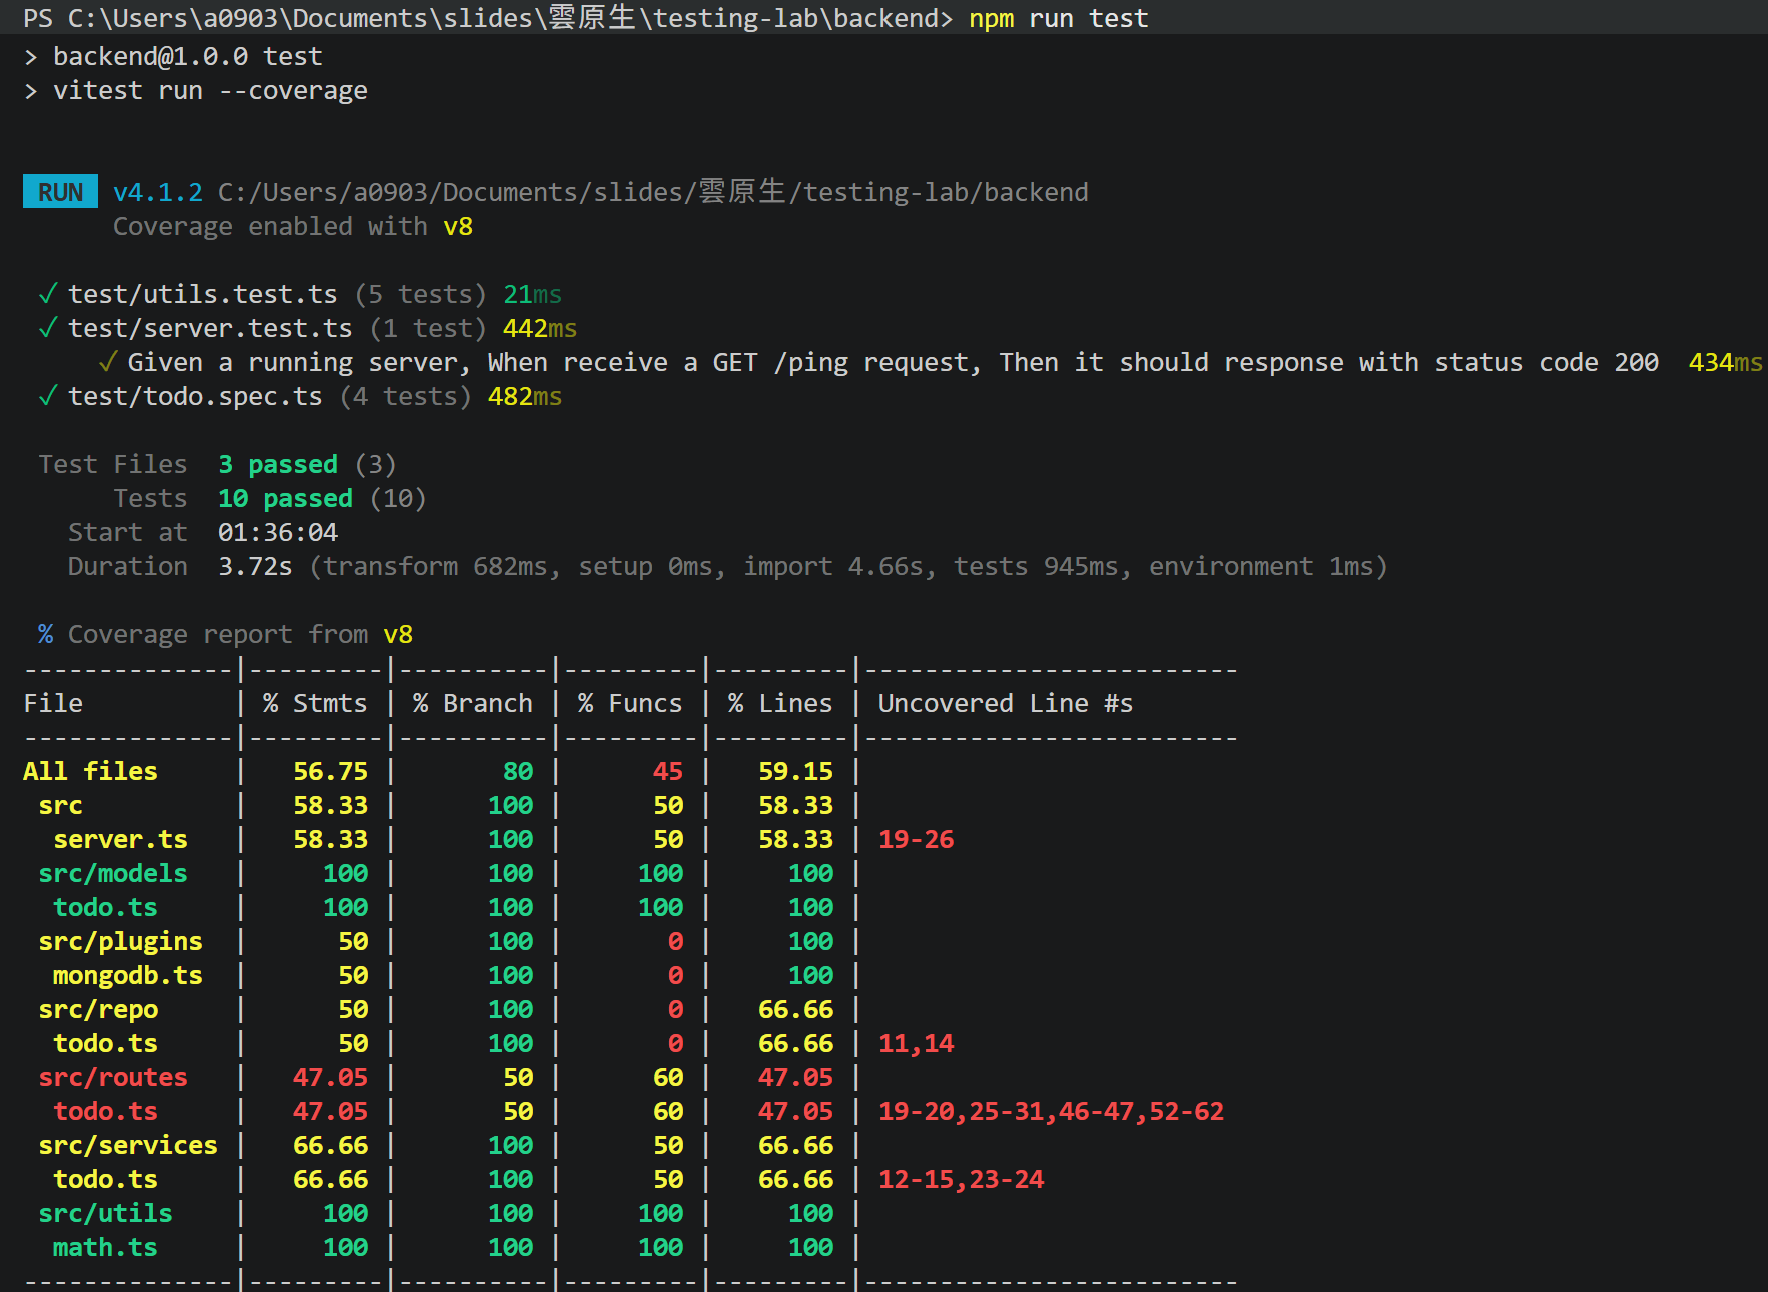
\includegraphics[width=0.8\textwidth]{todo.spec.ts_implement.png}
    \caption{todo.spec.ts測試報告}
    \label{fig:todo_test_report}
\end{figure}


\end{document}